\documentclass[aspectratio=169,10pt]{beamer}

% Minimal, editorial-style Beamer foundation
\usetheme{default}
\usefonttheme{professionalfonts}
\setbeamertemplate{navigation symbols}{}

\usepackage[utf8]{inputenc}
\usepackage[T1]{fontenc}
\usepackage[light,medium,sfdefault]{FiraSans}
\usepackage{ebgaramond}
\usepackage{FiraMono}
\usepackage{microtype}
\usepackage{graphicx}
\usepackage{booktabs}
\usepackage{colortbl}
\usepackage{listings}
\usepackage{xcolor}

% Light editorial palette with high-contrast, distinct accents
\definecolor{Ink}{HTML}{FAF9F6}          % warm off-white canvas
\definecolor{Graphite}{HTML}{EEF0F2}     % pale cool grey panels
\definecolor{Slate}{HTML}{E2E8ED}        % light blue-grey surfaces
\definecolor{Ivory}{HTML}{252B35}        % primary text
\definecolor{SoftIvory}{HTML}{46515F}    % secondary text
\definecolor{Muted}{HTML}{687382}        % captions and metadata
\definecolor{Champagne}{HTML}{B86B24}    % amber/orange accent
\definecolor{ChampagneLight}{HTML}{9A5B1D}
\definecolor{DustBlue}{HTML}{367FA6}     % blue accent
\definecolor{Sage}{HTML}{43866F}         % green accent
\definecolor{Clay}{HTML}{C65F4B}         % coral accent
\definecolor{PaleBlue}{HTML}{356F9A}
\definecolor{Violet}{HTML}{8060A8}       % lavender accent
\definecolor{Teal}{HTML}{25877F}         % teal accent

\setbeamercolor{normal text}{fg=Ivory,bg=Ink}
\setbeamercolor{structure}{fg=Teal}
\setbeamercolor{title}{fg=ChampagneLight}
\setbeamercolor{subtitle}{fg=Muted}
\setbeamercolor{author}{fg=SoftIvory}
\setbeamercolor{frametitle}{fg= DustBlue,bg=Ink}
\setbeamercolor{framesubtitle}{fg=Muted,bg=Ink}
\setbeamercolor{itemize item}{fg=Teal}
\setbeamercolor{itemize subitem}{fg=Muted}
\setbeamercolor{enumerate item}{fg=Champagne}
\setbeamercolor{section in toc}{fg=Ivory}
\setbeamercolor{subsection in toc}{fg=Muted}
\setbeamercolor{block title}{fg=Ink,bg=Teal}
\setbeamercolor{block body}{fg=Ivory,bg=Graphite}
\setbeamercolor{block title alerted}{fg=Ink,bg=Clay}
\setbeamercolor{block body alerted}{fg=Ivory,bg=Graphite}
\setbeamercolor{block title example}{fg=Ink,bg=Violet}
\setbeamercolor{block body example}{fg=Ivory,bg=Graphite}
\setbeamercolor{caption name}{fg=DustBlue}
\setbeamercolor{author in head/foot}{fg=Muted,bg=Ink}
\setbeamercolor{page number in head/foot}{fg=Muted,bg=Ink}

% Quiet title hierarchy and restrained page numbering
\setbeamerfont{title}{family=\rmfamily,size=\LARGE,series=\mdseries}
\setbeamerfont{subtitle}{size=\normalsize,series=\mdseries}
\setbeamerfont{frametitle}{family=\rmfamily,size=\Large,series=\mdseries}
\setbeamerfont{framesubtitle}{family=\sffamily,size=\scriptsize,series=\mdseries}
\setbeamerfont{normal text}{family=\rmfamily,size=\small,series=\mdseries}
\setbeamerfont{itemize/enumerate body}{family=\rmfamily}
\setbeamerfont{itemize/enumerate subbody}{family=\rmfamily}
\setbeamertemplate{frametitle}{%
  \vspace{0.35em}%
  \begin{beamercolorbox}[wd=\paperwidth,ht=2.5ex,dp=1.1ex,leftskip=0.65cm,rightskip=0.5cm]{frametitle}%
    \usebeamerfont{frametitle}\insertframetitle
  \end{beamercolorbox}%
  \ifx\insertframesubtitle\empty\else%
    \begin{beamercolorbox}[wd=\paperwidth,ht=1.7ex,dp=0.6ex,leftskip=0.65cm]{framesubtitle}%
      \usebeamerfont{framesubtitle}\insertframesubtitle
    \end{beamercolorbox}%
  \fi
}
\setbeamertemplate{footline}{%
  \begin{beamercolorbox}[wd=\paperwidth,ht=2.6ex,dp=1.1ex,rightskip=0.55cm]{page number in head/foot}%
    \hfill\usebeamerfont{page number in head/foot}\insertframenumber\hspace{0.15em}/\hspace{0.15em}\inserttotalframenumber
  \end{beamercolorbox}%
}
\setbeamertemplate{itemize item}{\raise0.15ex\hbox{\small\textcolor{Sage}{\textbullet}}}
\setbeamertemplate{itemize subitem}{\raise0.1ex\hbox{\scriptsize\textcolor{DustBlue}{\textbullet}}}
\setbeamertemplate{sections/subsections in toc}[sections numbered]
\setlength{\parskip}{0.15em}

% --- packages and helpers needed by the Backend slides (taken from slides/beamer_Backend.tex) ---
\usepackage{tabularx}
\usepackage{array}
\usepackage{tikz}
\usetikzlibrary{arrows.meta,positioning,calc}
\usepackage{ragged2e}

\newcolumntype{L}[1]{>{\RaggedRight\arraybackslash}p{#1}}
\newcolumntype{Y}{>{\RaggedRight\arraybackslash}X}
\setlength{\tabcolsep}{5pt}
\arrayrulecolor{Muted}
\renewcommand{\arraystretch}{1.12}

\lstset{
  basicstyle=\ttfamily\scriptsize\color{SoftIvory},
  keywordstyle=\bfseries\color{ChampagneLight},
  commentstyle=\itshape\color{Muted},
  stringstyle=\color{Champagne},
  backgroundcolor=\color{Graphite},
  frame=single,
  rulecolor=\color{Slate},
  breaklines=true,
  showstringspaces=false
}


\tikzset{
  box/.style={draw=#1,thick,rounded corners=3pt,fill=Graphite,text=Ivory,align=center,
              inner sep=3pt,text width=2.9cm,minimum height=0.85cm},
  arr/.style={-{Stealth},thick,draw=Muted}
}
\title[SysMon]{Alerts System}
\author{}\institute{}\date{}

\begin{document}
\setbeamertemplate{itemize item}{\raise0.1ex\hbox{\scriptsize\textcolor{Sage}{\textbullet}}}

% ===================== SLIDE 1 =====================
\begin{frame}{Alert Engine (\texttt{src/alerts.py})}{How a threshold rule turns into an alert}
\centering
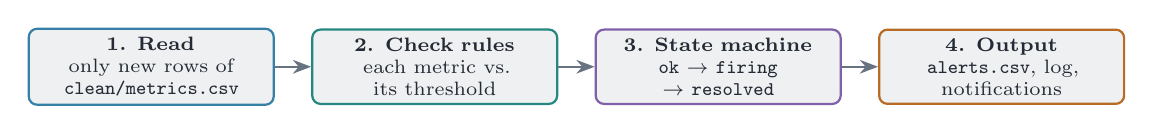
\begin{tikzpicture}[font=\scriptsize]
\node[box=DustBlue] (a) at (0,0) {\textbf{1. Read}\\only new rows of\\\texttt{clean/metrics.csv}};
\node[box=Teal]     (b) at (3.6,0) {\textbf{2. Check rules}\\each metric vs.\\its threshold};
\node[box=Violet]   (c) at (7.2,0) {\textbf{3. State machine}\\\texttt{ok} $\rightarrow$ \texttt{firing}\\$\rightarrow$ \texttt{resolved}};
\node[box=Champagne](d) at (10.8,0){\textbf{4. Output}\\\texttt{alerts.csv}, log,\\notifications};
\draw[arr] (a)--(b); \draw[arr] (b)--(c); \draw[arr] (c)--(d);
\end{tikzpicture}

\vspace{0.3em}
\footnotesize
\begin{columns}[T]
\begin{column}{0.49\textwidth}
\textbf{Rules} (\texttt{config/thresholds.conf})
\begin{itemize}
  \item 9 metrics: CPU, memory, swap, disk, load, CPU/GPU temp, GPU use.
  \item Per rule: \texttt{metric, op, threshold, severity} (warning / critical).
  \item \textbf{\texttt{sustained}}: breaches in a row needed $\Rightarrow$ ignores one-off spikes.
  \item \textbf{\texttt{cooldown\_s}}: minimum gap between repeats.
  \item \textbf{\texttt{no\_data}}: critical if no sample for $>60$\,s (collector down).
  \item Defaults scale to hardware (load $=2\times$ cores); invalid rules are skipped.
\end{itemize}
\end{column}
\begin{column}{0.49\textwidth}
\textbf{Evaluation logic}
\begin{itemize}
  \item \textbf{Fire:} breach count $\ge$ \texttt{sustained} and cooldown over.
  \item \textbf{Resolve:} first value back in range; counter resets.
  \item \textbf{Data-quality aware:} long gaps reset the count; filled/empty values are ignored.
  \item \textbf{Incremental:} state in \texttt{alert\_state.json}; reads only new rows.
  \item \textbf{Context:} logs the top CPU process at that moment.
\end{itemize}
\begin{block}{Example}
\texttt{cpu\_high}: $>85\%$ for 3 samples $\Rightarrow$ firing.
\end{block}
\end{column}
\end{columns}
\end{frame}

% ===================== SLIDE 2 =====================
\begin{frame}{Alert Delivery, Dashboard and Reliability}{From alert event to the user}
\footnotesize
\begin{columns}[T]
\begin{column}{0.32\textwidth}
\textbf{Delivery}
\begin{itemize}
  \item Runs as stage 3 of \texttt{run\_pipeline.sh}; can be switched off with \texttt{alerts\_enabled}.
  \item Notifies on \textit{firing} only, and only for events $<5$\,min old.
  \item Channels: desktop popup + sound; optional email (SMTP) and Telegram via env variables.
  \item A failed channel is logged and never stops the engine.
\end{itemize}
\end{column}
\begin{column}{0.34\textwidth}
\textbf{Dashboard \& API}
\begin{itemize}
  \item \texttt{alerts.csv}: one row per event (time, rule, value, threshold, severity, state, process).
  \item Alerts page: filter by state/severity, live badge, pop-up toasts.
  \item \texttt{/api/alerts}: list, \texttt{ack}, \texttt{resolve}, \texttt{clear}, \texttt{test}.
  \item Rules edited in Settings via \texttt{/api/config} (validated).
\end{itemize}
\end{column}
\begin{column}{0.30\textwidth}
\textbf{Reliability}
\begin{itemize}
  \item Atomic writes for state and config; alert rows appended in one write.
  \item Rule validation: allow-listed metrics and operators.
  \item \texttt{-{}-test} sends a fake alert through every channel.
  \item 27 unit tests (\texttt{test\_alerts.py}).
\end{itemize}
\end{column}
\end{columns}

\vspace{0.4em}
\begin{block}{Verified on real telemetry}
Under sustained load: \textbf{warning at 80$^\circ$C}, \textbf{critical at 90$^\circ$C}, auto-\textbf{resolved at 77$^\circ$C}.
\end{block}
\end{frame}

\end{document}
